\section{Executable forecasts with uncertain fill moments}
\label{sec:productionforecast}

The random-fill calculation identifies the appropriate signal but leaves
three practical questions: how to handle uncertainty in every moment,
how to retain price and quantity grids, and how to transfer a conditional
expected gain to realized random-filled outcomes. This section answers
those questions in explicit finite or bounded cells, without assuming
that a predicted target is fully executed.

\subsection{The label is tied to the action and the receipt clock}

For an order instruction $j$ sent at local time $t$, define all features
from $\mathcal G_t$, the information available after receipt and sequence
recovery. The instruction specifies side, venue, price, size, lifetime and
cancellation policy. A label for its value must preserve the association
between each executed quantity, its execution price and its markout horizon.
For example, its execution contribution marked at $T$ is
\[
 Y^{\rm exec}_j=\sum_{i\in\mathcal F_j}
 \varepsilon_j f_i(S_T-P_i)-\sum_{i\in\mathcal F_j}\mathrm{fee}_i,
\]
where $\varepsilon_j=1$ for buys and $-1$ for sells, $f_i\ge0$, and
$\mathcal F_j$ is the set of that instruction's actual fills. Carried
inventory and hedge costs are separate terms. This is a terminal markout,
not a claim that every filled position is liquidated at $S_T$ without cost.
Cash liquidation requires its executable price and fee.

A midpoint return measured from signal time is generally a different label.
Changing $j$ changes the distribution of fills and marks. Training a single
unconditional return forecast and multiplying by an unconditional fill rate
therefore needs an independence argument. Using exchange time for features
that arrived after $t$ violates the information constraint even if the
recorded event time is earlier than the decision. Training labels may be
realized later, but feature construction may not read them.

\subsection{All-moment uncertainty and physically consistent fills}

Retain the one-period assumptions of Section~\ref{sec:randomexecution}:
initial holding $b$, order increment $u$, fixed joint law of
$(\Phi,R)$ within a given instruction cell, proportional charge $c\ge0$,
position coefficient $a>0$ and order coefficient $\kappa\ge0$.
Let $\theta=(p,s,m)$ denote
$\E\Phi$, $\E\Phi^2$ and $\E[\Phi R]$. The moment restrictions
\[
 0\le p\le1,\qquad p^2\le s\le p
\]
follow from Jensen's inequality and $0\le\Phi\le1$.
If $|R|\le R_{\max}$ then $|m|\le R_{\max}p$, though these inequalities
alone need not characterize the joint family one intends to admit.
Use a nonempty compact convex moment set $\mathcal U$ derived from a
common joint-law family, or state explicitly that it is an outer relaxation.
Define
\begin{equation}\label{eq:allmomentgain}
 \underline G(u)=\inf_{(p,s,m)\in\mathcal U}
 \left\{um-abpu-cp|u|-\tfrac12(as+\kappa)u^2\right\}.
\end{equation}
The initial holding contributes uncertainty through $p$ as well as through
$m$. A plug-in estimate of $p$ or $s$ does not inherit the earlier
mean-only uncertainty guarantee.

\begin{proposition}[Robust decisions with uncertain execution moments]
\label{prop:allmoments}
Let $K$ be a compact interval containing zero. If
$as+\kappa\ge h_0>0$ throughout $\mathcal U$, then
$\underline G$ is continuous and $h_0$-strongly concave on $K$.
It has a unique maximizer $u_R$ and
\[
 \underline G(u_R)\ge0,\qquad
 \underline G(u_R)\ge\tfrac12h_0u_R^2.
\]
If $\mathcal U$ is a polytope, its inner infimum is attained at a vertex.
For a finite feasible lot grid $K_{\rm lot}$ containing zero, enumerating
$\underline G$ on that grid gives an exact robust discrete maximizer
with nonnegative guaranteed gain; uniqueness on the grid is not asserted.
\end{proposition}
\begin{proof}
For each $\theta$, the objective plus $h_0u^2/2$ is concave because
$cp\ge0$ and $as+\kappa\ge h_0$. An infimum of concave functions is
concave, proving strong concavity. Compactness of $\mathcal U$ and uniform
continuity on $K\times\mathcal U$ prove continuity of the infimum.
Compactness gives attainment and strong concavity gives uniqueness.
The feasible zero has value zero. The strong-concavity inequality between
$u_R$ and zero, followed by a limit along their segment, gives the quadratic
lower bound. The inner expression is affine in $(p,s,m)$ at fixed $u$,
so a compact polytope attains its minimum at a vertex. Finite enumeration
and inclusion of zero prove the discrete claim.
\end{proof}

For positive candidate orders the right derivative at zero is
\[
 \underline G'_+(0)=\inf_{\theta\in\mathcal U}\{m-abp-cp\}.
\]
Thus, on $K=[0,U]$ with $U>0$, no buy is robustly optimal exactly when
this infimum is nonpositive. For a two-sided interval with zero interior,
zero is optimal exactly when that condition and
$\sup_{\theta\in\mathcal U}\{m-abp+cp\}\ge0$ both hold.
These are directional derivative conditions for a concave function;
there need not be one common worst-case parameter at both signs.
If buy and sell orders have different laws, use separate one-sided
instruction cells and compare their certified values with zero.

\subsection{An exact joint-scenario implementation}

Let scenarios $z_j=(\phi_j,r_j)$ have an unknown probability vector
$w$ in a compact polytope
\[
 \mathcal W=\{w\ge0:\boldsymbol1^\top w=1,\quad Aw\le d\}.
\]
For each permitted order $u$, evaluate the linear programme
\begin{equation}\label{eq:scenarioLP}
 \underline G(u)=\min_{w\in\mathcal W}\sum_j w_j
 \left[u\phi_jr_j-ab\phi_ju-c\phi_j|u|
       -\tfrac a2\phi_j^2u^2-\tfrac\kappa2u^2\right].
\end{equation}
This construction automatically retains compatibility of all three moments.
An $\ell_1$ probability ball about empirical frequencies is representable
with auxiliary variables. Its radius requires valid coverage for the
joint sample, not separate accuracy claims for returns and fills.
If instruction laws depend on size, use a separately supported
$\mathcal W_u$ for each discrete action; the concavity conclusion across
$u$ no longer follows, but finite enumeration remains valid.

A numerical minimizer supplies an upper bound on the inner minimum and
therefore is not by itself a guaranteed lower gain. For an LP written as
$\min c_u^\top w$ subject to $Aw\le d$, $Ew=e$, $w\ge0$, a dual feasible
pair $y\le0,z$ with $A^\top y+E^\top z\le c_u$ gives the lower bound
$d^\top y+e^\top z$. Check feasibility with outward error allowances
before calling the result certified. The supplement independently compares
floating-point LP results with exact vertex values in its two-law rational
example; general floating-point optimizer outputs remain numerical checks.

In the earlier binary-fill example, admit mixtures of the independent and
adverse laws with adverse weight $\theta\in[0,0.2]$. Then
$p=s=0.5$, $m\in[0.01,0.02]$, $a=0.10$, $c=0.01$, $b=0$ and
$\kappa=0$. The robust continuous buy is $u_R=0.10$ with guaranteed gain
$0.00025$. On the lot grid $\{0,0.08,0.16,\ldots,0.96\}$, the exact
robust decision is $0.08$ with gain $0.00024$. The worst-case law is the
same endpoint for all positive orders. This example makes both uncertainty
and lot granularity visible without adding an empirical claim.

\subsection{Pathwise exposure in a multi-order portfolio}\label{sec:fillbox}

Let orders $u_i$ have componentwise fill fractions $\phi_i\in[0,1]$ and
resulting position $b+D_\phi u$, where $D_\phi$ is diagonal. For a linear
exposure limit $h^\top(b+D_\phi u)\le L$, the robust condition is exactly
\begin{equation}\label{eq:fillboxexposure}
 h^\top b+\sum_i\max(h_i u_i,0)\le L.
\end{equation}
Indeed each independent box coordinate maximizes its linear term at zero
or one. This is an exposure bound over possible fills, not an independence
assumption on their probabilities. Add a corresponding inequality for
each side of every risk limit and include outstanding orders from prior
decisions. If fill support is more restrictive, its support function can
replace the box bound. Checking only expected positions can violate a hard
limit even when the mean is far inside it.

The quadratic moment matrix $\E[D_\phi^{\mathsf T}AD_\phi]+K$ retains
cross-asset fill dependence. A diagonal approximation needs its own operator
error allowance. Shared funding and hedging obligations can also couple
otherwise separate instruments. Integer order selection under these limits
is a finite constrained optimization problem; componentwise clipping of an
unconstrained portfolio need not solve it.

\subsection{A realized-gain certificate for random-filled orders}

At sequential decision $t$, let $b_t,u_t,a_t,c_t,\kappa_t$ be predictable,
and let the one-period realized improvement over retaining $b_t$ be
\begin{equation}\label{eq:filledY}
 Y_t=u_t\Phi_tR_t-a_tb_tu_t\Phi_t-c_t|u_t|\Phi_t
       -\tfrac12a_tu_t^2\Phi_t^2-\tfrac12\kappa_tu_t^2.
\end{equation}
An evaluation period settles this payoff before the next period's outcome
is revealed. Overlapping labels require a different filtration or batching
argument. The benchmark here retains the current $b_t$ within each cell;
the sum is not automatically the difference from one separately evolving
baseline portfolio. Such a comparison needs its own accounting and
counterfactual coupling.

Suppose a simultaneous moment-coverage event of probability at least
$1-\delta_c$ implies $\mu_t:=\E[Y_t\mid\mathcal G_{t-1}]\ge g_t$
for every $t$, where $g_t$ is the predictable certified gain of the selected
order. The conditional noise must be controlled for $Y_t$, including the
random fill and risk terms, rather than only for $R_t$.

\begin{corollary}[Time-uniform transfer for filled-order gains]\label{thm:filledsequential}
Assume predictable bounds $\underline y_t\le Y_t\le\overline y_t$ hold almost surely, write
$W_t=\overline y_t-\underline y_t$ and $V_n=\sum_{t\le n}W_t^2/4$, and suppose a coverage event of
probability at least $1-\delta_c$ implies
$\mu_t:=\mathbb E[Y_t\mid\mathcal G_{t-1}]\ge g_t$ for every $t$. For fixed
$\rho>0$ and $0<\delta_m<1$, with probability at least $1-\delta_c-\delta_m$,
simultaneously for all $n\ge1$, \begin{equation}\label{eq:filledboundary}
 \sum_{t\le n}Y_t\ge\sum_{t\le n}g_t-
 \sqrt{(V_n+\rho)\log\!\left(\frac{V_n+\rho}{\rho\delta_m^2}\right)}.
\end{equation}
\end{corollary}

\begin{proof}
Hoeffding's lemma gives
$\mathbb E[e^{\lambda(Y_t-\mu_t)}\mid\mathcal G_{t-1}]\le e^{\lambda^2W_t^2/8}$
for every real $\lambda$, which is \eqref{eq:predictablesubgaussian} with $v_t=W_t^2/4$ for
$\xi_t=Y_t-\mu_t$. By Remark~\ref{rem:sequential-general},
Theorem~\ref{thm:sequentialgain} applies with $v_0=\rho$ and $\alpha=\delta_m$; its
boundary $B_{\delta_m}(V_n)$ is the deviation term in \eqref{eq:filledboundary}.
\end{proof}


This is a bounded-outcome application of the normal-mixture construction,
not a new confidence-sequence method \citep{HowardEtAl2021}. One sufficient
conservative bound, when $|R_t|\le R_{\max}$, $|b_t|\le B$ and
$|u_t|\le U$, is $|Y_t|\le M_t$, with
\[
 M_t=UR_{\max}+a_tBU+c_tU+\tfrac12(a_t+\kappa_t)U^2,
 \qquad W_t=2M_t.
\]
For unbounded returns replace this by a proved conditional exponential
moment bound, or account for truncation bias and tails. A normal-mixture
formula cannot be made valid merely by substituting an empirical variance.
Coverage error and realized-noise error are distinct probabilities.

\subsection{Experiments and an implementable evaluation contract}

\begin{table}[htbp]
\centering\small
\caption{Synthetic random-fill implementation checks. Gains use the
risk-penalized units of \eqref{eq:allmomentgain}, not cash backtest returns.}
\begin{tabular}{p{.57\linewidth}r}
\toprule
Quantity & Value\\\midrule
\inputtable{tables/production_rows.tex}
\bottomrule
\end{tabular}
\end{table}

The supplement compares joint-scenario linear programmes against exact
endpoint calculations, enumerates finite lot choices and fill-box vertices,
and checks the conditional noise inequality directly for discrete laws.
It also enumerates short sequential outcome trees for the mixture boundary.
Those computations are diagnostics; the all-time statement is established
by the supermartingale proof, not by finite simulation.

A meaningful market evaluation freezes the features, order instructions,
markout horizons, cost conventions and selection rule before testing.
Split by chronological sessions; purge training labels whose outcome
windows overlap the test period. Assess fill-weighted moments, conditional
marks and selected order values, including no-fill and canceled orders.
Report calibration and value by action support, signal age and market regime.
Show actual net cash outcomes separately from risk-adjusted scores and
from the confidence lower bound. Paper~I's execution interface supplies the
separate parent-completion problem; prediction quality alone does not
supply a guaranteed completion mechanism.


\begin{figure}[htbp]
\centering
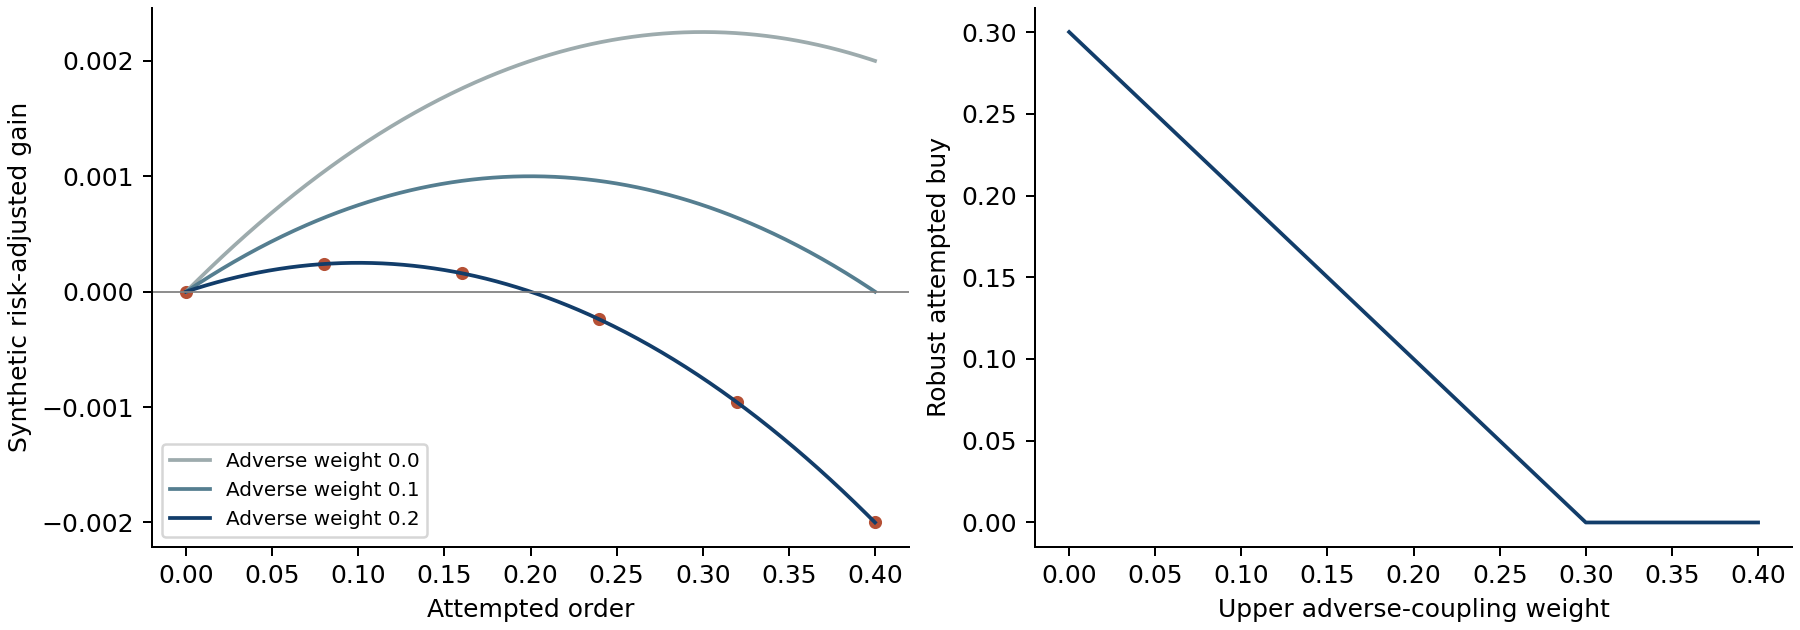
\includegraphics[width=\linewidth]{figures/07_production_bridge.png}
\caption{Discrete implementation diagnostics generated by the accompanying
reference suite. All axes use synthetic model units; the curves illustrate
the declared mechanisms rather than estimated market behavior.}
\label{fig:productionbridge}
\end{figure}

\subsection{Heterogeneous horizons and representation crowding}
A finite irreducible continuous-time chain is exponentially mixing.
To approximate persistent flow of the kind derived by
\citet{RodriguezDominguez2026Switching} over a fitted horizon, the contraction rate $\omega$ in
\eqref{eq:spanmixing} must be compatible with that observed decay. The forecast certificates of Section~5 can conservatively use $\omega=0$,
$C_0(h)=h^2/2$, unless a rate is separately verified.
\citet{RodriguezDominguez2026Market} makes the conditioning representation itself an
equilibrium object. For Theorem~\ref{thm:nonlinearinformation} this bears on one
hypothesis: it compares information classes under a fixed law of the future
increment, whereas a representation adopted widely enough to move prices changes
that law.

